\section{Observations and Motivation} % just find the problem and benefit
\label{sec:background}

\subsection{Need for Deduplication}

The proliferation of Containers and Container platforms has resulted in an explosion of the number of Docker images.
In order to understand the extent of storage requirements and performance demands from a Docker registry, 
we observe the amount of public repositories hosted by Docker Hub registry. 
We chose the Docker Hub registry~\cite{docker-hub} as our source of images due to its popularity 
and its significant number of public repositories. 
%%
%Docker Hub does not provide an API to retrieve all repository names.
%Hence, we crawled the registry's website to obtain a list of all available
%repositories, and then downloaded the \emph{latest} version of an image and its
%corresponding layers for each repository.
% over a period of 30 days.
%
%We plan to extend our analysis to other image tags in the future.
%
%We downloaded 355,319 images, resulting in 1,792,609 compressed layers
%and 5,278,465,130 files, with a total compressed dataset size of 47\,TB.
%
%
%To store and analyze the data, we deployed an 8-node Spark~\cite{spark}
%cluster with HDFS~\cite{hdfs} as the backend storage.
%%
We noticed that the number of public repositories is constantly increasing with a growth that amounts 
to around 1 million repositories annually. 
This corresponds to~130\,TB of annual growth in storage needs \HA{but it is actually less because of shared layers, right?}, 
costing around~\$15,000 a month if Google Cloud Storage is used~\cite{GoogleCloudStoragePricing}.
This growth implies significant benefits to data deduplication. 

We further performed an in-depth and empirical analysis of the viability of deduplication on container images. 
We analyzed around 50\,TB of compressed Docker images collected from Docker Hub. 
In order to provide insights in terms of the redundancy measure in the image dataset and the benefits of deduplication,
we have to first decompress the layers included in the images. 
The decompressed layer comprises a set of files. 
The total number of files we observed amount to over 5 billion files.
%Remarkably, only around 3\%\HA{3\% or 7\% ?} of the those files are unique while the rest are redundant copies. 
%This suggests that the current layer sharing strategy that Docker already employs is not efficient in eliminating duplicate data. 
%Further investigations on the causes for the high number of redundant files exposed a few findings. 
%For example, different Docker images often contain the same 
%source code from external public repositories like GitHub~\cite{github}.
%This is because no official images contain this source code, 
%so users manually add it to their images, 
%resulting in different layers which cannot be reused.


\paragraph{Deduplication statistics} % the potential of deduplication 

%%%%layer ref count 
%
A remarkable observation that emerges from the data analysis is that only around 3\%\HA{3\% or 7\% ?} of the layers' constituent files are unique while the rest are redundant copies. 
This suggests that the current layer sharing strategy that Docker already employs is not efficient in eliminating duplicate data. 
We further analyzed the repeat count for every file and plotted the distributions as shown in Figure~\ref{fig:file-repeat-cnt}.
We found that over 99.4\% of files have more than one copy.
Around 50\% of files have exactly 4 copies and 90\% of files have 10 or less copies. 
This indicates the high potential for file-level deduplication in the Docker registry.

%\begin{figure} \centering
%	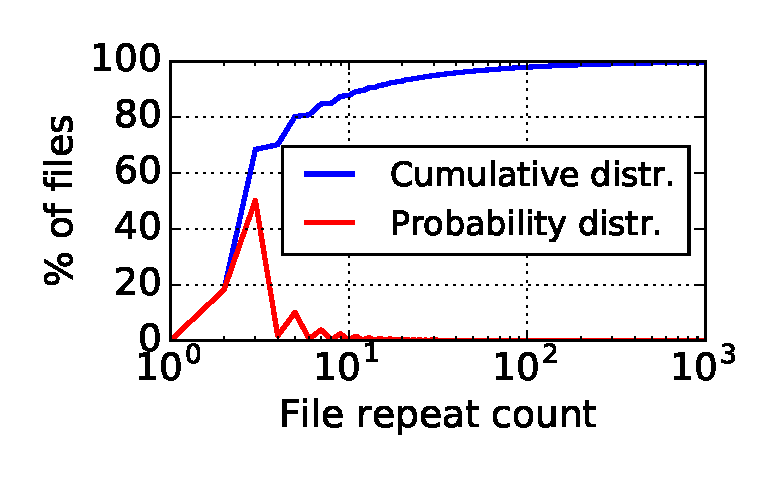
\includegraphics[width=0.45\textwidth]{graphs/File_repeat_count.eps}
%	\caption{File repeat count distribution.
%	%
%	\VT{No need for Y2}
%	%
%	\VT{Still need to use \% on the axis}\NZ{addressed both}
%	%
%	} \label{fig:file-repeat-cnt}
%\end{figure}

\begin{figure}[t]
	\centering
	\begin{minipage}{0.35\textwidth}
		\centering
		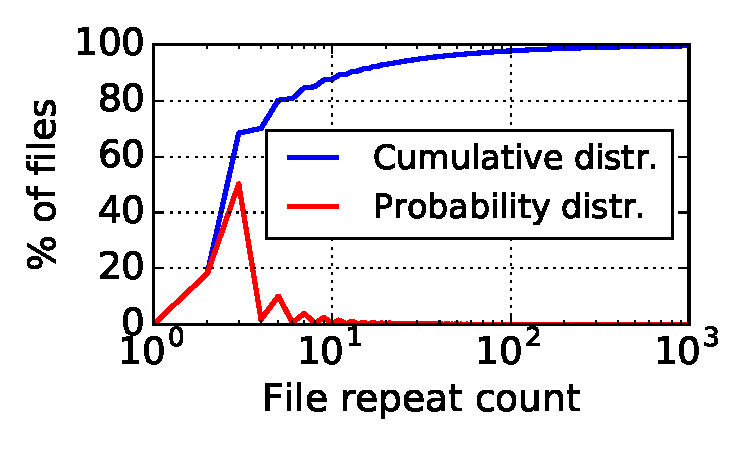
\includegraphics[width=1\textwidth]{graphs/File_repeat_count-eps.pdf}
		\caption{File repeat count distribution.
		}
		%\vspace{15pt}
		\label{fig:file-repeat-cnt}
	\end{minipage}
	\begin{minipage}{0.35\textwidth}
		\centering
		%\vspace{-10pt}
		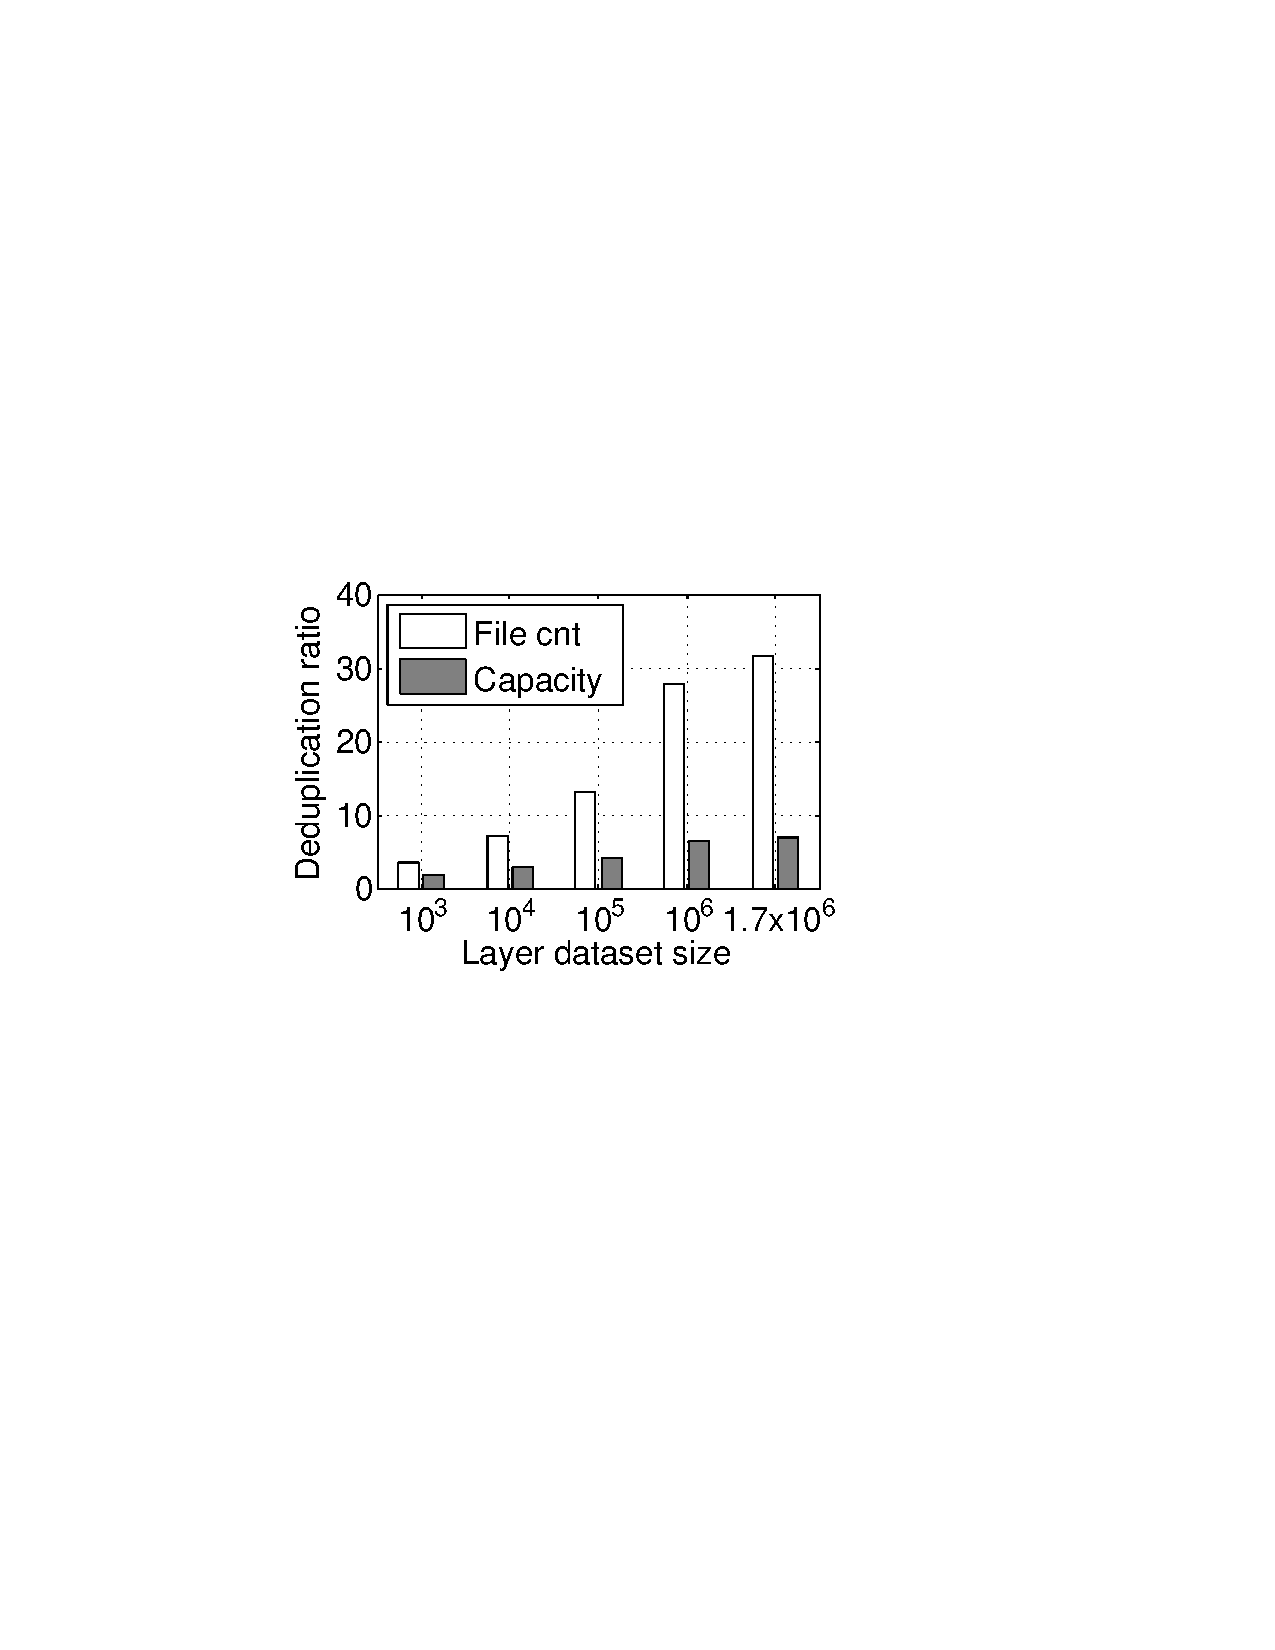
\includegraphics[width=1\textwidth]{graphs/dedup-ratio-grow} 
		\caption{Deduplication ratio growth.
		} 
		\vspace{-2pt}
		\label{fig:dedup-ratio-growth}
	\end{minipage}
\end{figure}

%\begin{figure} 
%	\centering
%	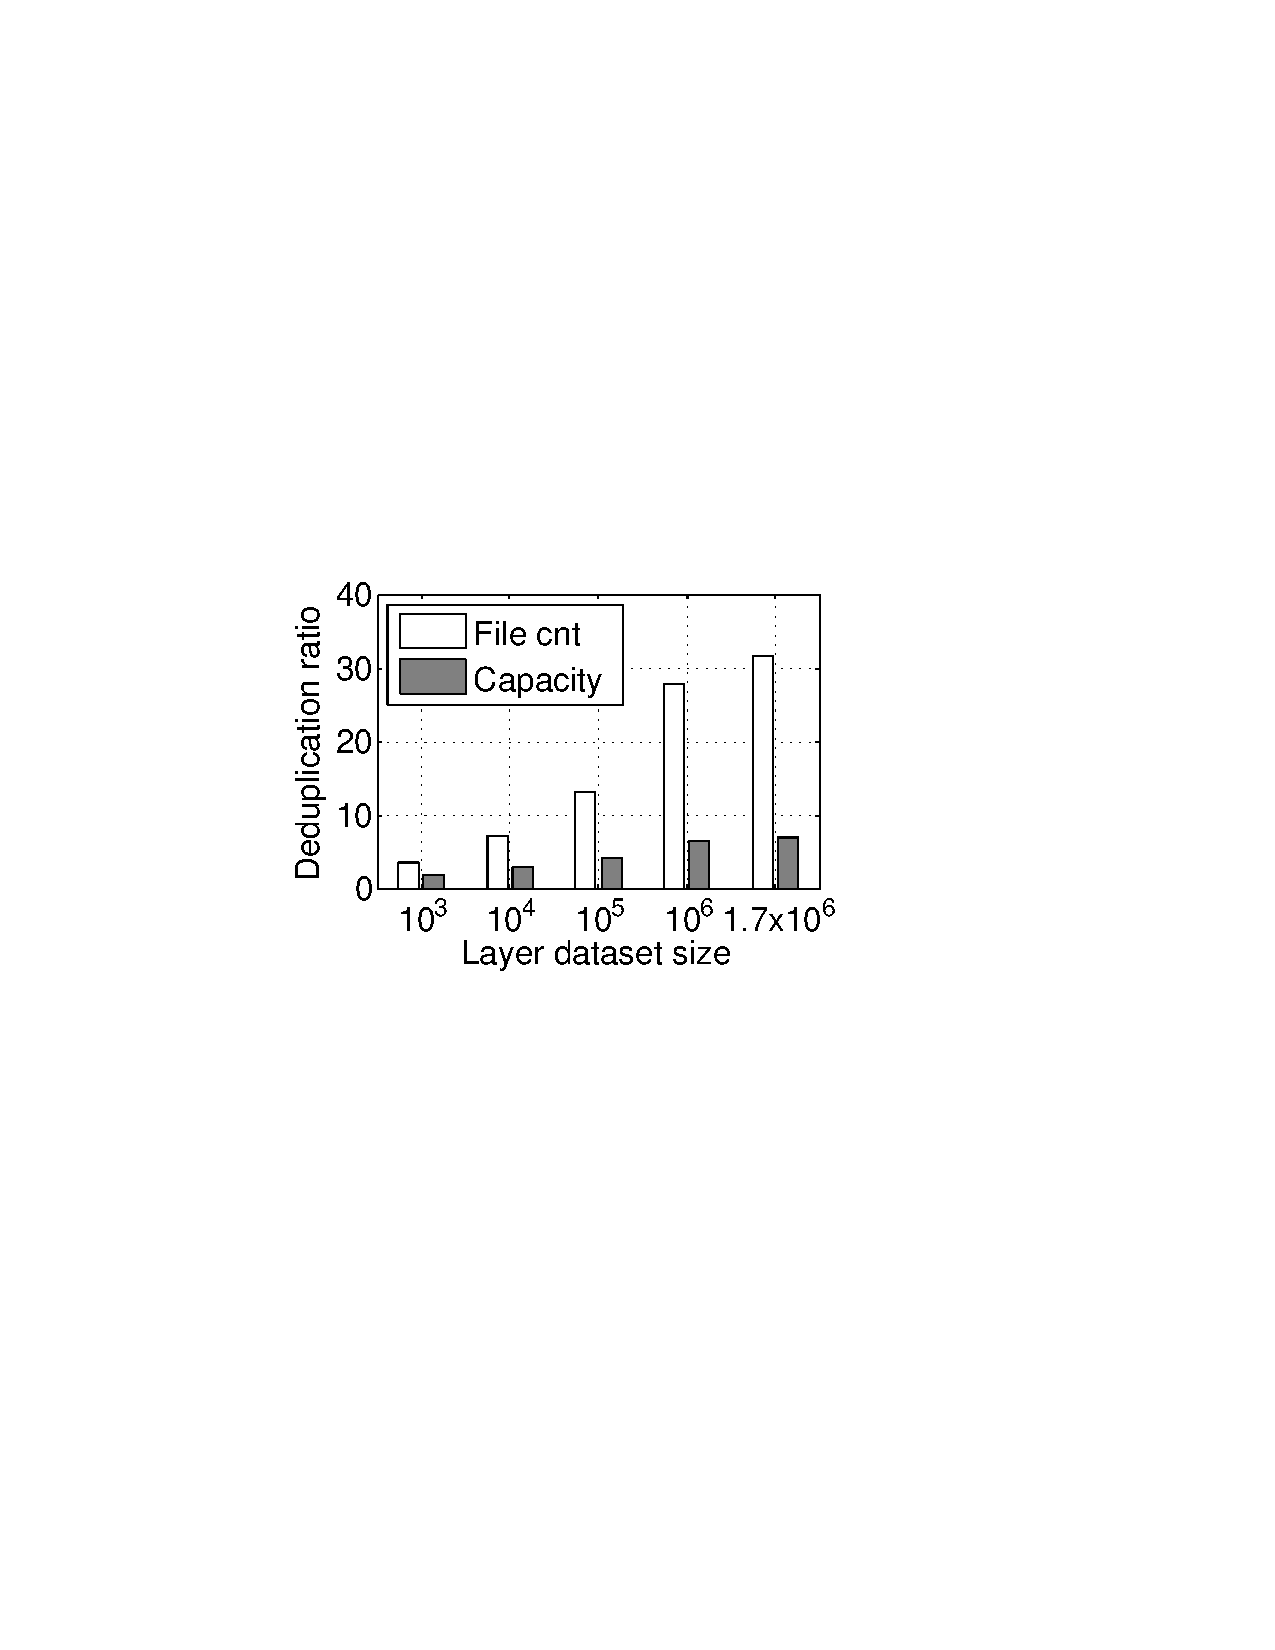
\includegraphics[width=0.25\textwidth]{graphs/dedup-ratio-grow} 
%	\caption{The growth of deduplication ratio.
%	} 
%	\label{fig:dedup-ratio-growth} 
%\end{figure}



\paragraph{Deduplication ratio growth} % benefit
%
Further investigations on the potential of file-level deduplication involved analyzing the deduplication ratio. 
As shown in Figure~\ref{fig:dedup-ratio-growth}, we analyzed the deduplication 
ratio and its growth for an increasing number of files stored in the registry.   
%(see Figure~\ref{fig:dedup-ratio-growth}).
%
%Figure~\ref{fig:dedup-ratio-growth} shows the deduplication ratio growth over the layer dataset size. 
%
The x-axis values correspond to the sizes of 4 random samples drawn from the whole dataset and the size of the
whole dataset.

We see that the deduplication ratio increases almost linearly with the layer dataset size.
This implies that the benefits of file-level deduplication strengthens as the number of public repositories and images grow.
%
%As the number of images stored in the Docker registry increases dramatically,
%file-level deduplication can provide significant storage space savings.



%\subsection{Need for Usr-oriented cache management}
%
%\paragraph{Access skewness}
%
%\paragraph{Reuse time distribution}
%
%\paragraph{Hit ratios}
%
%\paragraph{Hit ratios with prefetching}
%
%%\subsection{} % what are the cost for a naive file-level deduplication
%
%\paragraph{Restoring performance breakdown}